\documentclass[12pt]{article}
%\usepackage[document]{ragged2e}
\usepackage{array, amssymb, amsthm, linguex, enumerate, amsmath, physics, enumitem, xcolor, graphicx, xparse}
\let\fg\undefined %remove linguex/siunitx naming clash
\usepackage[english]{babel}
\usepackage[letterpaper,top=2cm,bottom=2cm,left=3cm,right=3cm,marginparwidth=1.75cm]{geometry}
\usepackage[colorlinks=true, allcolors=blue]{hyperref}
\usepackage[group-separator={,}]{siunitx} %\num{12345} -> "12,345"
\usepackage{fancyhdr}
\usepackage{listings}
\usepackage{notomath}
\usepackage[T1]{fontenc}
%Number sets
\newcommand{\R}{\mathbb{R}}
\newcommand{\C}{\mathbb{C}}
\newcommand{\N}{\mathbb{N}}
\newcommand{\F}{\mathbb{F}}
\renewcommand{\Re}{\operatorname{Re}}
\renewcommand{\Im}{\operatorname{Im}}
\renewcommand{\L}[1]{\mathcal{L}\left({#1}\right)} %Linear Map

\newcommand{\pmp}{\,\pm\,} %add small extra space to \pm

\NewDocumentCommand{\ceil}{ s m }{% ceiling brackets
    \IfBooleanTF{#1}%
    {\lceil #2 \rceil}% starred: no-autosizing
    {\left\lceil #2 \right\rceil}% unstarred: autosizing
}

\NewDocumentCommand{\ceiling}{ s m }{% ceiling brackets
    \IfBooleanTF{#1}%
    {\lceil #2 \rceil}% starred: no-autosizing
    {\left\lceil #2 \right\rceil}% unstarred: autosizing
}

\NewDocumentCommand{\floor}{ s m }{% floor brackets
    \IfBooleanTF{#1}%
    {\lfloor #2 \rfloor}% starred: no-autosizing
    {\left\lfloor #2 \right\rfloor}% unstarred: autosizing
}

\NewDocumentCommand{\pars}{ s m }{% parenthesis
    \IfBooleanTF{#1}%
    {( #2 ) }% starred: no-autosizing
    {\left( #2 \right) }% unstarred: autosizing
}

\NewDocumentCommand{\inner}{ s m }{% inner product
    \IfBooleanTF{#1}%
    {\langle #2 \rangle}% starred: no-autosizing
    {\left\langle #2 \right\rangle}% unstarred: autosizing
}

\NewDocumentCommand{\brac}{ s m }{% brackets
    \IfBooleanTF{#1}%
    {[#2] }% starred: no-autosizing
    {\left[ #2 \right] }% unstarred: autosizing
}

%default latex bracket size naming
\newcommand{\biggbrac}[1]{\bigg[ {#1} \bigg] }
\newcommand{\bigbrac}[1]{\big[ {#1} \big] }
\newcommand{\Bigbrac}[1]{\Big[ {#1} \Big] }


\RenewDocumentCommand{\over}{ s m }{% fraction 1/arg
    \IfBooleanTF{#1}%
    {\dfrac{1}{#2}}% starred: dfrac
    {\frac{1}{#2}}% unstarred: normal frac
}

\NewDocumentCommand{\pover}{ s m }{% parenthesis around fraction (1/arg)
    \IfBooleanTF{#1}%
    {\left(\dfrac{1}{#2}\right)}% starred: dfrac
    {\left(\frac{1}{#2}\right)}% unstarred: normal frac
}

\NewDocumentCommand{\pfrac}{ s m m}{% parenthesis around fraction (arg1/arg2)
    \IfBooleanTF{#1}%
    {\left( \dfrac{{#2}}{{#3}} \right)}% starred: dfrac
    {\left( \frac{{#2}}{{#3}} \right)}% unstarred: normal frac
}


\newcommand{\Xbar}{\bar{X}}
\newcommand{\Ybar}{\bar{Y}}
\newcommand{\xbar}{\bar{x}}
\newcommand{\ybar}{\bar{y}}


\newcommand{\limn}{\lim_{n\to\infty}}

\newcommand{\gammaDist}[2]{\operatorname{Gamma} \left( {#1},{#2} \right)} %gamma distribution
\NewDocumentCommand{\normalDist}{s g g}{ %normal distibution
    \IfBooleanTF{#1} { % starred, no autosizing parenthesis
      \IfNoValueTF{#2}{ 
          N (\mu,\, \sigma^2 ) %\normalDist* "default" normal distribution N(\mu, \sigma^2)
        } {
            \IfNoValueTF{#3}{N (#2)}{} %\normalDist{arg} --> N(arg)
        }
      \IfNoValueTF{#3}{}{N ( #2, #3 )}  %\normalDist*{arg1}{arg2} --> N(arg1,arg2)
    }  % else (unstarred) autosize parenthesis
    {
        \IfNoValueTF{#2}{
            N \left(\mu,\, \sigma^2 \right) %\normalDist "default" normal distribution N(\mu, \sigma^2)
        } {
            \IfNoValueTF{#3}{N \left(#2\right)}{} %\normalDist{arg} --> N(arg)
        }
        \IfNoValueTF{#3}{}{N \left( #2, #3 \right)} %\normalDist{arg1}{arg2} --> N(arg1,arg2)
    }
}



%colors
\definecolor{ggreen}{RGB}{0, 127, 0}
\definecolor{dgray}{RGB}{63,63,63}
\definecolor{neonorange}{RGB}{255,47,0}
\definecolor{mygray}{rgb}{0.5,0.5,0.5}
\definecolor{eblue}{RGB}{0,74,127}
\newcommand{\red}[1]{\color{red}{#1}\color{black}}
\newcommand{\green}[1]{\color{ggreen}{#1}\color{black}}
\newcommand{\blue}[1]{\color{blue}{#1}\color{black}}
\newcommand{\setRed}{\color{red}}
\newcommand{\setBlack}{\color{black}}
\newcommand{\setBlue}{\color{blue}}
\newcommand{\setGreen}{\color{ggreen}}



\newcommand{\thru}[1]{{#1}_1, \dots, {#1}_n}
\newcommand{\sumThru}[1]{{#1}_1 + \cdots + {#1}_n}
\newcommand{\yn}{Y_1, \dots, Y_n} % Y_1, ..., Y_n
\newcommand{\xn}{X_1, \dots, X_n} % Y_1, ..., Y_n

%hats and tildes
\newcommand{\that}{\widehat{\theta}} % theta hat
\newcommand{\phat}{\widehat{p}} % p hat
\newcommand{\qhat}{\widehat{q}} % p hat
\newcommand{\psihat}{\widehat{\psi}} % psi hat
\newcommand{\Psihat}{\widehat{\Psi}} % Psi hat
\newcommand{\ptilde}{\widetilde{p}} % psi tilde
\newcommand{\Psitil}{\widetilde{\Psi}} % Psi tilde
\newcommand{\betah}{\widehat{\beta}} % beta hat
\newcommand{\muh}{\widehat{\mu}} % beta hat

%2x2 matrix shortcuts
\newcommand{\detx}[4]{\begin{vmatrix}{#1} & {#2}\\{#3}&{#4}\end{vmatrix}} % 2x2 determinant
\newcommand{\bmat}[4]{\begin{bmatrix}{#1} & {#2}\\{#3}&{#4}\end{bmatrix}} % 2x2 matrix brackets
\renewcommand{\pmat}[4]{\begin{pmatrix}{#1} & {#2}\\{#3}&{#4}\end{pmatrix}} % 2x2 matrix parenthesis

%remove any enumerate/itemize indent temporarily
\makeatletter   %% <- make @ usable in macro names
\newcommand*\notab[1]{%
  \begingroup   %% <- limit scope of the following changes
    \par        %% <- start a new paragraph
    \@totalleftmargin=0pt \linewidth=\columnwidth
    %% ^^ let other commands know that the margins have been reset
    \parshape 0
    %% ^^ reset the margins
    #1\par      %% <- insert #1 and end this paragraph
  \endgroup
}
\makeatother    %% <- revert @


\newcommand{\dimrange}[1]{\operatorname{dim}\operatorname{range}{#1}} % dimrange
\newcommand{\dimnull}[1]{\operatorname{dim}\operatorname{null}{#1}} % dimnull
\newcommand{\range}[1]{\operatorname{range}{#1}} %range
\newcommand{\nullspace}{\operatorname{null}} %null

% polynomial notation
\NewDocumentCommand{\poly}{ s g g }{%
    \IfBooleanTF{#1} {
        \IfNoValueTF{#2} {
            \mathcal{P}(\mathbb{R})
        } {
            \mathcal{P}_{#2}(\mathbb{R})
        }
    } {
        \IfNoValueTF{#3} {
            {\mathcal{P}(#2)}
        } { %else
            {\mathcal{P}_{#2}(#3)}
        }
    }
}

\NewDocumentCommand{\bias}{ s m }{% bias(arg)
    \IfBooleanTF{#1}%
    {\operatorname{bias}(#2)}% starred: no autosizing
    {\operatorname{bias}\left(#2\right)}% unstarred: autosizing
}

\NewDocumentCommand{\MSE}{ s m }{% MSE(arg)
    \IfBooleanTF{#1}%
    {\operatorname{MSE}(#2)}% starred: no autosizing
    {\operatorname{MSE}\left(#2\right)}% unstarred: autosizing
}

\NewDocumentCommand{\Var}{ s m }{% variance with parenthesis V(arg)
    \IfBooleanTF{#1}%
    {\operatorname{Var}(#2)}% starred: no autosizing
    {\operatorname{Var}\left(#2\right)}% unstarred: autosizing
}

\NewDocumentCommand{\Varb}{ s m }{% variance with brackets V[arg]
    \IfBooleanTF{#1}%
    {\operatorname{Var}[\,#2\,]}% starred: no autosizing
    {\operatorname{Var}\left[\,#2\,\right]}% unstarred: has autosizing
}

\NewDocumentCommand{\Vb}{ s m }{% another renaming of variance with brackets V[arg]
    \IfBooleanTF{#1}%
    {\operatorname{Var}[\,#2\,]}% starred: no autosizing
    {\operatorname{Var}\left[\,#2\,\right]}% unstarred: has autosizing
}

\NewDocumentCommand{\E}{ s m }{% expectation with parenthesis E(arg)
    \IfBooleanTF{#1}%
    {\operatorname{E}(#2)}% starred: no autosizing
    {\operatorname{E}\left(#2\right)}% unstarred: has autosizing
}

\NewDocumentCommand{\Eb}{ s m }{% expectation with brackets E[arg]
    \IfBooleanTF{#1}%
    {\operatorname{E}[#2]}% starred: no autosizing
    {\operatorname{E}\left[#2\right]}% unstarred: has autosizing
}

\RenewDocumentCommand{\P}{ s m }{% probability with parenthesis Pr(arg)
    \IfBooleanTF{#1}%
    {\Pr (#2) }% starred: no autosizing
    {\Pr \left( #2 \right) }% unstarred: has autosizing
}

\NewDocumentCommand{\prob}{ s m }{% probability with parenthesis Pr(arg)
    \IfBooleanTF{#1}%
    {\Pr (#2) }% starred: no autosizing
    {\Pr \left( #2 \right) }% unstarred: has autosizing
}

\NewDocumentCommand{\eff}{ s m }{% efficiency with parenthesis eff(arg)
    \IfBooleanTF{#1}%
    {\operatorname{eff}(#2)}% starred: no autosizing
    {\operatorname{eff}\left(#2\right)}% unstarred: has autosizing
}

%vertical vector of up to 8 elements
\NewDocumentCommand\vvec{s m g g g g g g g}{%
    \IfBooleanTF{#1} {
        \begin{bmatrix}% if starred use brackets
            \IfNoValueTF{#2}{}{#2}
            \IfNoValueTF{#3}{}{\\#3}
            \IfNoValueTF{#4}{}{\\#4}
            \IfNoValueTF{#5}{}{\\#5}
            \IfNoValueTF{#6}{}{\\#6}
            \IfNoValueTF{#7}{}{\\#7}
            \IfNoValueTF{#8}{}{\\#8}
        \end{bmatrix}
    }  % else (unstarred) use parethesis
    {
        \begin{pmatrix}%
            \IfNoValueTF{#2}{}{#2}
            \IfNoValueTF{#3}{}{\\#3}
            \IfNoValueTF{#4}{}{\\#4}
            \IfNoValueTF{#5}{}{\\#5}
            \IfNoValueTF{#6}{}{\\#6}
            \IfNoValueTF{#7}{}{\\#7}
            \IfNoValueTF{#8}{}{\\#8}
        \end{pmatrix}
    }
}
\def\Cov{\operatorname{Cov}} %Covariance
\def\df{\text{df}} %degrees of freedom

\NewDocumentCommand{\example}{ s g }{% Example header
    \IfBooleanTF{#1}%
    {\vspace{0.1in}}% starred: 0.1in
    {\vspace{0.2in}}% unstarred: 0.2in
    \IfNoValueTF{#2} {\noindent\textbf{\color{eblue} Example: }}{\noindent\textbf{\color{eblue} Example (#2): }}
}
\NewDocumentCommand{\disc}{ s }{% Discussion header
    \IfBooleanTF{#1}%
    {\vspace{0.1in}\noindent\textbf{Discussion: } }% starred: 0.1in
    {\vspace{0.2in}\noindent\textbf{Discussion: } }% unstarred: 0.2in
}
\NewDocumentCommand{\defn}{ s }{% Definition header
    \IfBooleanTF{#1}%
    {\vspace{0.1in}\noindent\textbf{\color{neonorange} Definition: } }% starred: 0.1in
    {\vspace{0.2in}\noindent\textbf{\color{neonorange} Definition: } }% unstarred: 0.2in
}
\NewDocumentCommand{\reason}{ s }{% Reason header
    \IfBooleanTF{#1}%
    {\vspace{0.1in}\noindent\textbf{Reason:} }% starred: 0.1in
    {\vspace{0.2in}\noindent\textbf{Reason:} }% unstarred: 0.2in
}
\NewDocumentCommand{\recall}{ s }{% Recall header
    \IfBooleanTF{#1}%
    {\vspace{0.1in}\noindent\textit{Recall:} }% starred: 0.1in
    {\vspace{0.2in}\noindent\textit{Recall:} }% unstarred: 0.2in
}
\NewDocumentCommand{\remark}{ s }{% Remark header
    \IfBooleanTF{#1}%
    {\vspace{0.1in}\noindent\textit{Remark:} }% starred: 0.1in
    {\vspace{0.2in}\noindent\textit{Remark:} }% unstarred: 0.2in
}
\NewDocumentCommand{\soln}{ s }{% Remark header
    \IfBooleanTF{#1}%
    {\vspace{0.1in}\noindent\textbf{Solution:} }% starred: 0.1in
    {\vspace{0.2in}\noindent\textbf{Solution:} }% unstarred: 0.2in
}

\newcommand{\proj}[2]{\operatorname{proj}_{{#1}}{#2}} %projection
\newcommand{\wideand}{\qquad \text{and} \qquad}

\newcommand{\bu}[1]{\textbf{\underline{{#1}}} } %bold underline
\newcommand{\boldit}[1]{\textbf{\textit{{#1}}} } %bold italix

% put actual quotation marks "around something"
\newcommand{\say}[1]{\textquotedblleft{#1}\textquotedblright}

% max{arg} and min{arg}
\renewcommand{\max}[1]{\operatorname{max}\left\{ #1 \right\}}
\renewcommand{\min}[1]{\operatorname{min}\left\{ #1 \right\}}

%circle around argument
\newcommand{\cir}[1]{\textcircled{\raisebox{-1pt}{#1}}}

% Updates the current chapter number.
% 0 based indices
\newcommand{\setChapter}[1]{
    \setcounter{chapter}{#1}
    \setcounter{section}{0}
}


% Code snippets
\newcommand{\code}[1]{{\fontfamily{qcr}\selectfont #1}}

\lstset{
    backgroundcolor=\color{white},
    basicstyle=\fontfamily{qcr}\footnotesize,
    breakatwhitespace=false,         % sets if automatic breaks should only happen at whitespace
    breaklines=true,                 % sets automatic line breaking
    captionpos=b,                    % sets the caption-position to bottom
    commentstyle=\color{dgray},    % comment style
    deletekeywords={...},            % if you want to delete keywords from the given language
    escapeinside={(*@}{@*)},          % if you want to add LaTeX within your code
    extendedchars=true,              % lets you use non-ASCII characters; for 8-bits encodings only, does not work with UTF-8
    firstnumber=1,                % start line enumeration with line 1
    frame=single,	                   % adds a frame around the code
    keepspaces=true,                 % keeps spaces in text, useful for keeping indentation of code (possibly needs columns=flexible)
    keywordstyle=\color{ggreen}\bfseries,       % keyword style
    language=SQL,                 % the language of the code
    morekeywords={*,...},            % if you want to add more keywords to the set
    numbers=left,                    % where to put the line-numbers; possible values are (none, left, right)
    numbersep=5pt,                   % how far the line-numbers are from the code
    numberstyle=\tiny\color{mygray}, % the style that is used for the line-numbers
    rulecolor=\color{black},         % if not set, the frame-color may be changed on line-breaks within not-black text (e.g. comments (green here))
    showspaces=false,                % show spaces everywhere adding particular underscores; it overrides 'showstringspaces'
    showstringspaces=false,          % underline spaces within strings only
    showtabs=false,                  % show tabs within strings adding particular underscores
    stringstyle=\bfseries\color{darkorange},     % string literal style
    tabsize=4	                   % sets default tabsize to 4 spaces
}

\lstdefinestyle{cpp}{language=C++,
    morekeywords={cout, cin, Comparable, T},numbers=none,
    basicstyle=\fontfamily{qcr}\scriptsize
}

\lstdefinestyle{sql}{
    language=sql,
    numbers=none,
    commentstyle=\color{ggreen},
    frame=none,
    keywords=[1]{SET, LEFT, OUTER, SELECT, UPDATE, DELETE, INSERT, INTO, FROM, GROUP, BY, INNER, JOIN, WHERE, DISTINCT, VALUES},
    keywordstyle=\bfseries,
    keywordstyle=[1]\color{eblue}\bfseries,
    keywords=[2]{AS, ON, NOT, AND, OR, IN, IS, NULL},
    keywordstyle=[2]\color{brightblue}\bfseries,
    keywords=[3]{COUNT, MAX, SUM, MIN},
    keywordstyle=[3]\color{purp}\bfseries,
    keywords=[4]{Eats, Person, Serves, Frequents, EMPLOYEE, WORKS\_ON, DEPENDENT, DEPT\_LOCATIONS, DEPARTMENT, PROJECT},
    keywordstyle=[4]\color{purp},
    keywords=[5]{name, age, gender, pizzeria, pizza, price, Fname, Lname, Ssn, Dno, Essn, Relationship, Dname, Dnumber, Mgr\_ssn, Mgr\_start\_date, Dlocation, Pno, Hours, Pname, Pnumber, Plocation, Dnum, Minit, Bdate, Address, Sex, Salary, Super\_ssn, Dependent\_name},
    keywordstyle=[5]\color{mediumblue}
}


% Update global section number, O based indices
\newcommand{\setSection}[1]{\setcounter{section}{#1}}



%Set table of contents depth
\setcounter{tocdepth}{3}


%Create a new vspace line no indent
\newcommand{\nl}{\vspace{0.1in}\noindent}
\newcommand{\nnl}{\vspace{0.2in}\noindent}
\newcommand{\nnnl}{\vspace{0.3in}\noindent}

%Remove hyphens
\tolerance=1
\emergencystretch=\maxdimen
\hyphenpenalty=10000
\hbadness=10000

\textwidth=7.02in
\hoffset=-.45in



\setcounter{MaxMatrixCols}{20}
\begin{document}

\pagestyle{fancy}
\fancyhf{}
\fancyhead[RO]{Matthew Wilder} %header top right
\fancyhead[LO]{MTH 326 - Homework \#8} %header top left
\fancyfoot[CO]{Page \thepage} %page center bottom

\noindent MTH 326 - Spring 2022
\\Assignment \#9
\\Due: Friday, April 29 2022 (11:59pm)

\begin{enumerate}
    \item Suppose the following represents a random sample of points $(x,y)$:
\notab{\begin{center}
    \begin{tabular}{|c|c|c|c|c|c|} 
         \hline
         $x$ & -2 & -1 & 0 & 1 & 2\\
         \hline
         $y$ & 3 & 2 & 1 & 1 & 0.5\\
         \hline
    \end{tabular}
\end{center}}

\begin{enumerate}[label={(\alph*)}]
    \item Find the 90\% confidence interval for $\E{Y}$ when $x^* = 0$ and again when $x^* = 2$.

\nnl \textbf{Solution: } For a 90\% CI then $\alpha = 1 - 0.9 = 0.1$ and a two sided is $\alpha/2 = 0.05$. There are $n-2$ degrees of freedom, hence $\df = 5-2 = 3$. Therefore $t_{\alpha/2}(\df) = t_{0.05}(3) = 2.353.$ We want to use the following formula,
$$\pars{\widehat{\beta_0} + \widehat{\beta_1} x^*} \, \pm \, t_{\alpha/2}(\text{df})S \displaystyle \sqrt{\over{n} + \dfrac{\pars{x^* - \bar x}^2}{S_{xx}}}$$
so we need to compute the remaining unknows. It is trivial that $\xbar = 0$ and $\ybar = 1.5$. Then
$$S_{xx} = \sum (x_i-\xbar)^2 = \sum x_i^2 = 4 + 1 + 0 + 1 + 4 = 10$$
$$S_{yy} = \sum (y_i-\ybar)^2 = \sum (y_i-1.5)^2 =  (1.5)^2 + (0.5)^2 + 2(-0.5)^2 + (-1)^2 = 4$$
and 
$$S_{xy} = \sum (x_i-\xbar)(y_i-\ybar) = \sum x_i(y_i-1.5) = -2(1.5) - (0.5) + (-0.5) + 2(-1) = -6.$$
Then 
$$\betah_1 = \frac{S_{xy}}{S_{xx}} = \frac{-6}{10} = -0.6$$
and
$$\betah_0 = \ybar - \betah_1 \xbar = 1.5.$$
Then
$$S = \sqrt{\dfrac{\operatorname{SSE}}{n-2}} =  \sqrt{ \dfrac{S_{yy} - \betah_1 S_{xy}} {n-2}} = \sqrt{ \dfrac{4- (-0.6 \cdot -6)}{3} } = \sqrt{\frac{0.4}{3}} \approx  0.365148.$$
Therefore our inverval is
$$(1.5 - 0.6x^*) \pm 2.353\cdot  0.365148 \sqrt{\over{5} + \frac{(x^*)^2}{10}}$$
so for $x^* = 0$ then 
$$1.5 \pm 2.353\cdot  0.365148 \sqrt{\over{5}} \equiv (1.116, 1.884)$$
and for $x^* = 2$ then 
$$(1.5 - 0.6(2) ) \pm 2.353\cdot  0.365148 \sqrt{\over{5} + \frac{(2)^2}{10}} \equiv (-0.366, 0.966).$$
    \item Find the 90\% confidence interval for $Y^*$ when $x^* = 0$ and again when $x^* = 2$.

\nnl \textbf{Solution: } We adjust the interval to 
$$(1.5 - 0.6x^*) \pm 2.353\cdot  0.365148 \sqrt{{\setRed 1} + \over{5} + \frac{(x^*)^2}{10}}$$
so for $x^* = 0$ then 
$$1.5 \pm 2.353\cdot  0.365148 \sqrt{1 + \over{5}} \equiv (0.5588, 2.4412)$$
and for $x^* = 2$ then 
$$(1.5 - 0.6(2) ) \pm 2.353\cdot  0.365148 \sqrt{1 + \over{5} + \frac{(2)^2}{10}} \equiv (-0.7868, 1.3868).$$\vspace{1in}
    \item Are the intervals for $\E{Y}$ or the intervals for $Y^*$ wider? How can this be explained?

\nnl \textbf{Solution: } The intervals for $Y^*$ are wider than $\E{Y}$ because the $(\betah_0 + \betah_1x^*)$ is held constant as the center of the interval, then the scalar $t_{\alpha/2}(\df)S$ is a fixed constant. Lastly, the scalar value under the squareroot is positive since $\frac{1}{n} > 0$, $(x^*-\xbar)^2 > 0 \, \forall \, x \in \R$, and $S_{xx} > 0$ since its also squares.  Adding positive values together is stilll positive. Hence adding another positive number (+1) to this value results in a larger positive value. Therefore the squareroot of the new positive value is also larger. Hence the scalar around the center of the interval is larger (\say{wider}).

\notab{
$$\overbrace{\pars{\widehat{\beta_0} + \widehat{\beta_1} x^*} \, \pm \, t_{\alpha/2}(\text{df})S \displaystyle \sqrt{\over{n} + \dfrac{\pars{x^* - \bar x}^2}{S_{xx}}}}^{\textstyle \E{Y}} < \overbrace{\pars{\widehat{\beta_0} + \widehat{\beta_1} x^*} \, \pm \, t_{\alpha/2}(\text{df})S \displaystyle \sqrt{1 + \over{n} + \dfrac{\pars{x^* - \bar x}^2}{S_{xx}}}}^{\textstyle Y^*}$$
$$\iff t_{\alpha/2}(\text{df})S \sqrt{\over{n} + \dfrac{\pars{x^* - \bar x}^2}{S_{xx}}} < t_{\alpha/2}(\text{df})S \sqrt{1 + \over{n} + \dfrac{\pars{x^* - \bar x}^2}{S_{xx}}}$$
$$\iff \sqrt{\underbrace{\over{n} + \dfrac{\pars{x^* - \bar x}^2}{S_{xx}}}_{> 0}} < \sqrt{1 + \underbrace{\over{n} + \dfrac{\pars{x^* - \bar x}^2}{S_{xx}}}_{>0}}$$}
\end{enumerate}\vspace{1in}
    \item Data is collected from three populations ($A$, $B$, $C$) which have normal distributions with a common variance. The data is as follows:
\notab{
    \begin{center}
    \begin{tabular}{|c|c c c|} 
        \hline
        A & 1 & 3 & 2\\
        B & 6 & 4 & \\
        C & 6 & 8 & 4\\
        \hline
   \end{tabular}\end{center}
}
\begin{enumerate}[label={(\alph*)}]
    \item This data set is small enough to do by hand. Determine $\widehat{\mu}_i$'s, $\widehat{\mu}_0$, $\operatorname{SSA}$ and $\operatorname{SSW}$.

\soln We have $k=3$, $n_1 = n_3 = 3$, $n_2 = 2$ and $n = 8$. Then
\begin{align*}
    \muh_1 &= \over{3} \bigbrac{1 + 3 + 2} = 2\\
    \muh_2 &= \over{2} \bigbrac{6 + 4} = 5\\
    \muh_3 &= \over{3} \bigbrac{6+8+4} = 6\\
    \muh_0 &= \over{n} \sum_{i=1}^{k} n_i \muh_i = \over{8} \bigbrac{3(2)+2(5)+3(6)} = 4.25\\
    \operatorname{SSA} &= \sum_{i=1}^k n_i (\muh_i - \muh_0)^2 = 3 (2 - 4.25)^2 + 2 (5 - 4.25)^2 + 3 (6 - 4.25)^2 = 25.5\\
    \operatorname{SSW} &= \sum_{i=1}^k \sum_{j=1}^{n_i} \pars{Y_{i\,j} - \muh_i}^2\\
    &= \underbrace {
        (1-2)^2 + (3-2)^2 + (2-2)^2
    }_{i=1}
    + \underbrace{
        (6-5)^2 + (4-5)^2
    }_{i=2} + \underbrace{
        (6-6)^2 + (8-6)^2 + (4-6)^2
    }_{i=3}
    = 12
\end{align*}
    \item Fill out the ANOVA table for this experiment.

\soln* 
\notab{
    \begin{center}
    \begin{tabular}{|l|c c c c c|} 
        \hline
        Source & SS & df & Mean Squares & $F_{\text{obs}}$ & $p$-value\\
        \hline
        among & 25.5 & 2 & 12.75 & 5.3125 & 0.057926\\
        within & 12 & 5 & 2.4 & &\\
        total & 37.5 & 7 & & &\\
        \hline
   \end{tabular}
\end{center}
}\newpage
    \item Is there sufficient evidence at level $\alpha = 0.10$ that at least one of the means is different from the others? Briefly explain.

\soln* Since $0.058 = p < \alpha = 0.1$ then we reject the null hypothesis. Hence, there \textit{is} evidence that at least one of the means are different. \vspace{0.3in}
    \item Give bounds for the $p$-value in this experiment.

\soln*$p \in (0.05, 0.1)$ by appendix table 7 since $F(2,5)_{.1} = 3.78 <F < F(2,5)_{.05} = 5.79$
\end{enumerate}\vspace{.5in}
    \item Students at a large high-school preparing for the ACT exam have the option of attending
an ACT tutorial session. Some students chose to do this and some do not. School
administrators want to determine if the tutorial helps. The ACT scores of students at
this school are summarized below:
\notab{\begin{center}
    \begin{tabular}{|r l l l|} 
         \hline
         attended tutorial: & $\ybar = 26$ & $S = 3.5$ & $n = 50$ \\
         did not attend: & $\ybar = 25$ & $S = 3$ & $n = 80$\\ 
         \hline
    \end{tabular}
\end{center}}
\begin{enumerate}[label={(\alph*)}]
    \item Determine $\widehat{\mu}_0$ and then compute $\operatorname{SSA}$ (or $\operatorname{SST}$, using the book's notation) and $\operatorname{SSW}$ (or $\operatorname{SSE}$) in the book.

\soln* 
\begin{align*}
    \muh_0 &= \over{n} \sum_{i=1}^{k} n_i \muh_i = \over{130} \bigbrac{50(26)+80(25)} = 25.3846154\\
    \operatorname{SSA} &= \sum_{i=1}^k n_i (\muh_i - \muh_0)^2 = 50 (26 - 25.3846154)^2 + 80 (25 - 25.3846154)^2 = 30.7692308\\
    \operatorname{SSW} &= (50 - 1)(3.5^2) + (80-1)(3^2) = 1311.25\\
\end{align*}\vspace{.2in}
    \item Fill out the ANOVA table and test the administrators' conjecture at the $\alpha =0.05$ significance level. Fully justify your conclusion.

\soln* 
\notab{
    \begin{center}
    \begin{tabular}{|l|c c c c c|} 
        \hline
        Source & SS & df & Mean Squares & $F_{\text{obs}}$ & $p$-value\\
        \hline
        among & 30.769 & 1 & 30.769 & 3.00361187 & 0.085488\\
        within & 1311.25 & 128 & 10.244 & &\\
        total & 1342.02 & 129 & & &\\
        \hline
   \end{tabular}
\end{center}
}
Let $H_0 : \mu_1 = \mu_2$ and $H_a : \mu_1 \neq \mu_2$. Then for $\alpha = 0.05$, computing $F_{0.05}(1, 128) = 3.9151$ by WebAssign technology. Since $F_{\text{obs}} < F = 3.9151$ then we accept $H_0$. There is not enough evidence to indicate a difference in ACT performance.\vspace{.2in}
    \item Determine a 95\% confidence interval for the difference in means.

\soln* Using Chapter 9 techniques, $\displaystyle \text{CI} \equiv (\muh_1 - \muh_2) \pm t_{\alpha/2}(\df)\sqrt{\frac{S_1}{n_1} + \frac{S_2}{n_2}}$. Hence
\begin{align*}
    \text{C.I.} &= (26 - 25) \pm t_{0.025}(129) \sqrt{ \frac{3.5^2}{50} + \frac{3^2}{80}}\\
    &= 1 \pm 1.960 \cdot 0.59791\\
    &\equiv (-0.1719, \; 2.1719) \text{ points}
\end{align*}
Using $\operatorname{MSW} \equiv S^2$ yields (as it should) about the same decimals. \vspace{0.2in}
    \item Explain how your answer in (b) supports your conclusion in (a).

\soln* Interpretting this as how (b) supports (c): Since we accept the null hypothesis in (b) it would make logical sense that $0 \in \text{CI}$ from (c).
\end{enumerate}\vspace{.8in}
    \item An experiment was conducted to compare the starch content of tomato plants grown in
sandy soil supplemented by one of four different nutrient packages, A, B, C, and D.
\notab{\begin{center}
    \begin{tabular}{|c|c c c c c c|} 
         \hline
         A & 45 & 47 & 67 & 61 & 56 & 72\\
         B & 39 & 39 & 43 & 46 & 59 & 27\\ 
         C & 60 & 42 & 55 & 44 & 30 & 18\\
         D & 56 & 61 & 60 & 47 & 69 & 42\\ \hline
    \end{tabular}
\end{center}}
\begin{enumerate}[label={(\alph*)}]
    \item Using the technology of your choice, construct an ANOVA table.

\soln* We're really banking on the fact that I programmed this correctly (problem 2 was the only test case):

\notab{
    \begin{center}
        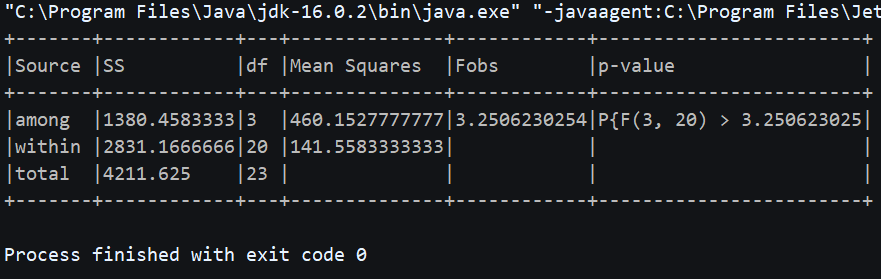
\includegraphics[width=6in]{problem4.png}
    \end{center}
}
    \item Report the $p$-value and interpret the $p$-value in the context of the problem

\soln* Computing the $p$-value (which I wasn't going to code or import an F-distibution) with the WebAssign technology, we get $p = 0.043377$. In the context of the problem we can be at most $95.66\%$ confident that at least one of the nutrient packages differs significantly from the others.
\end{enumerate}\newpage
    \item In class we stated the MLE for $\widehat{\mu}_i$ and ${S_a}^2$ under the alternative hypothesis that all the means are not equal. Using the likelihood function $L( \text{all } Y_{i\,j} \mid \widehat{\mu}_1 , \dots, \widehat{\mu}_k, {S_a}^2)$ that we derived in class, show that the MLE is as stated in class. (Hint: Recall that when using this method to determine $\that$, we differentiate with respect to the whole of the estimator $\displaystyle \pdv{\that}$)
    \item In class we stated that if $\displaystyle X \sim \chi^2 (n) = \Gamma\pars{ \frac{n}{2}, 2}$, so that the expected value of $\displaystyle \E{\over{X}} = \over{n-2}$. We seek to prove this.
\begin{enumerate}[label={(\alph*)}]
    \item Using the definition of the gamma function (the \textit{function}, not distribution), write
the following integral as a multiple of a gamma function:
\notab{
    $$\int_0^{\infty} x^{\frac{n}{2}-2}e^{-x/2} \, dx$$
    $$\text{Goal: }\, c\Gamma(z) = c\int_0^{\infty} x^{z-1} e^{-x}dx  \to \int_0^{\infty} x^{\frac{n}{2}-2}e^{-x/2}dx$$
}

\begin{align*}
    &\; \int_0^{\infty} x^{\frac{n}{2} -2} e^{-\frac{x}{2}} dx \tag{$u = \frac{x}{2}\; du = \over{2}dx$}\\
    =&\; \int_0^{\infty} (2u)^{\frac{n}{2} - 2} e^{-\frac{2u}{2}} (2du) \tag{apply $u$-sub}\\
    =&\; 2 \int_0^{\infty} 2^{\frac{n}{2} - 2} u^{\frac{n}{2} - 2} e^{-u} du \tag{pull constant \& distribute}\\
    =&\; 2^{\frac{n}{2} - 1} \int_0^{\infty} u^{\frac{n}{2} - 2} e^{-u} du \tag{pull new base 2 constant}\\
    =&\; 2^{\frac{n}{2}-1} \int_0^{\infty} u^{(\frac{n}{2} - 1) - 1} e^{-u} du \tag{linearity of addition}\\
    =&\; 2^{\frac{n}{2}-1} \, \Gamma\pars{\frac{n}{2} - 1} \tag{Gamma function substitution $z = \frac{n}{2} - 1$}
\end{align*}
Doing some factorial algebra, $\displaystyle \Gamma\pars{\frac{n}{2} - 1} = \frac{\Gamma\pars{\frac{n}{2}}}{n/2}$, so the above equals
$$\frac{2^{\frac{n}{2}-1}}{n/2} \Gamma \pars{\frac{n}{2}}.$$
    \item Via the definition, compute the expected value $\displaystyle \E{\over{X}}$.

\soln*
\begin{align*}
    \E{\over{X}} &= \int_0^{\infty} \over{x} f(x) dx \\
    &= \int_0^{\infty} \over{x}
        \pars{\over{\Gamma(\frac{n}{2}) 2^{\frac{n}{2}}}} x^{\frac{n}{2} - 1} e^{- \frac{x}{2}
    }
\\
    &=\over{\Gamma(\frac{n}{2}) 2^{\frac{n}{2}}} \int_0^{\infty} \over{x}
    x^{\frac{n}{2} - 1} e^{- \frac{x}{2}
}\\
&=\over{\Gamma(\frac{n}{2}) 2^{\frac{n}{2}}} \int_0^{\infty} 
x^{\frac{n}{2} - 2} e^{- \frac{x}{2}}\\
&=\over{\Gamma(\frac{n}{2}) 2^{\frac{n}{2}}}  \cdot  2^{\frac{n}{2}-1} \Gamma \pars{\frac{n}{2} - 1} \tag{substitution from (a)}\\
&= \over{(\frac{n}{2} - 1) \Gamma(\frac{n}{2} - 1) 2^{\frac{n}{2}}}  \cdot  2^{\frac{n}{2}-1} \Gamma \pars{\frac{n}{2} - 1}
\\ &= \over{n-2} \tag{\say{lots of killing} - (McAsey)}\\
\end{align*}
    \item Let $X_1 \sim \chi^2 (m)$ and $X_2 \sim \chi^2(n)$ be independent random variables. Define the random variable $F = \dfrac{X_1/m}{X_2/n}$. Use the previous results to compute the mean of $F$. (Note $F \sim F(m,n)$.)
\end{enumerate}\newpage
\end{enumerate}
$$Y = \beta_0 + \beta_1 x_1 + \beta_2 x_2 + \varepsilon$$
The data is as follows:
\notab{\begin{center}
    \begin{tabular}{|c|c|c|c|c|c|c|c|c|c|} 
         \hline
         $x_1$ & 2 & 1 & 1 & -3 & -1 & 0 & -2 & 0 & 2\\ \hline
         $x_2$ & -1 & 1 & -2 & 0 & 1 & 1 & 0 & -2 & 2\\ \hline
         $y$ & 3 & 6 & 5 & 8 & 12 & 7 & 4 & 11 & 10\\
          \hline
    \end{tabular}
\end{center}}

\begin{enumerate}[label=(\alph*)]
    \item Determine the matrices
    $\mathbf X, \;
    \mathbf X^T, \;
    \mathbf X^T\mathbf X,\;
    \mathbf X^T \mathbf Y, \text{ and } (\mathbf X^T\mathbf X)^{-1}$ \vspace{.1in}
    \item Fit the model to the data \vspace{.1in}
    \item Determine the residual for the data point $(1, 1, 6)$\vspace{.1in}
    \item Use matrices to calculate $\operatorname{SSE}$ and determine $S$. (Note $\sum y^2 = 564$.) \vspace{.1in}
    \item Test $H_0 : \beta_2 = 0$ versus $\beta_2 < 0$. Perform the test at $\alpha = 0.05$ level. What can you conclude about the usefulness of the $x_2$ term in the model? \vspace{.1in}
    \item Find a $99\%$ confidence interval for $\E{Y}$ when $x_1 = 1$ and $x_2 = 2$.
\end{enumerate}

\nnl $$\frac{\bigbrac{(600 * 1) + (300 * 4) + (100 * 2 )} * 10^3 }{\num{1000000}} = 2$$
$${\frac{2 \times 10^9}{2 \times 10^6} = 10^3 = 1000}$$
$$\underbrace{\num{1000000}}_{\text{IC}} \times \underbrace{\frac{2 \times 10^6}{2 \times 10^9}}_{\text{CPI / f}} = 1000 \mu \text{s}$$
\end{document} 